\chapter{Learning to valuate fluents in games}

\label{ch:fluents}

% TODO: par about grounding?

In Chapter~\ref{ch:rl}, we've presented how to apply Deep Reinforcement
Learning to achieve non-Markovian goals. We've seen that a construction based
on temporal logics, that we call the Restraining Bolt, is an elegant solution
that transforms the original problem to a classic MDP, by producing additional
rewards and observations. We report the general scheme here, in
Figure~\ref{fig:rb-focus-features}.
\begin{figure}
	\centering
	\begin{tikzpicture}[
			every node/.append style={font=\small},
			arrow/.style={->, semithick},
		]
		\matrix [
			 row sep=0.5cm, column sep=1cm,
		] {
			\node (env) [block, minimum size=2cm] {World}; \& \& \&
			\node (agent) [block, minimum size=2cm] {Learning\\agent}; \\
			\&
			\node (features) [block, fill=lightgray] {Features\\extractor}; \&
			\node (rb) [block] {Restraining\\Bolt}; \& \\
		};
		\coordinate (a1) at ($(agent.west)+(0,0.5)$);
		\draw [arrow] (a1) -- node [near start, above] {$a$} (env.east |- a1);
		\coordinate (w1) at ($(env.east)+(0,-0.2)$);
		\draw [arrow] (w1) -- node [near start, above] {$r$} (agent.west |- w1);
		\coordinate (w2) at ($(env.east)+(0,-0.5)$);
		\draw [arrow] (w2) -- node [near start, below] {$o$} (agent.west |- w2);
		\draw [arrow] (w2) ++(0.5,0) |- (features.west);
		\draw [arrow] (features) -- node [near start, above] {$l$} (rb);
		\draw [arrow] ($(rb.east)+(0,0.1)$) -- ++(0.3,0)
			|- node [below right] {$\vec{q}$} ($(agent.west)+(0,-0.8)$);
		\draw [arrow, dashed] ($(rb.east)+(0,-0.1)$)
			-| node [near end,right] {$r'$} (agent.south);
	\end{tikzpicture}
	\caption{In this chapter, we focus on the features extractor.}
	\label{fig:rb-focus-features}
\end{figure}
The two blocks at the bottom are our additions, and part of the solution.
We've thoroughly addressed the Restraining Bolt in Section~\ref{sec:rb},
already. In this chapter, we want to focus on the other essential component:
the features extractor.

The purpose of the features extractor is to receive an observation from the
environment and produce a Boolean valuation for some predefined propositional
symbols, that we call fluents. We assume that the set of fluents~$\fluents$
has already been defined, and the truth of every atomic proposition
in~$\fluents$ can be decided from a single input~$o$. This means that if we
did define a symbol that cannot be decided from one observation, for example a
generic ``$\const{GoalReached}$'' condition, we need to split that symbol into
much simpler events, and define $\const{GoalReached}$ in terms of the new
fluents.

Usually, the features extractor is not a really interesting component. Once,
we've defined a fluent~$\fluent \in \fluents$, we could manually program a
function, $f_p: \obsS \to \B$, that predicts when that event occurs or that
condition is verified\footnote{$\B$ is the set $\set{0, 1}$, which represents
$\set{\false, \true}$.}.  This approach is perfectly fine, when applicable.
However, the environments used in Deep Reinforcement Learning usually produce
high-dimensional or noisy observations. As we may imagine, it becomes really
hard to manually classify such inputs in the two classes. So, in order to
apply the Restraining Bolt or any other logic-based method to Deep RL, we
must resort to some Machine Learning model that will help us deciding the
truth of our atomic propositions.

Any Deep RL agent processes the input observation with a Neural Network. A
reasonable choice would be to use a NN also as model for the features
extractor. We may use a joint network that predicts the value for every fluent
defined: $f: \obsS \to \B^{\abs{\fluents}}$. The simplest way to train this
model is through supervised learning, where we provide many input-output
samples. Supervised learning can generate very accurate models, but, for every
image in the training dataset, we would need to manually label the desired
outputs, i.e. the fluents that are true in that image. Unfortunately, the
effort of this manual intervention would completely dominate over the
advantages of the high-level, logic approach. If possible, we would certainly
like to avoid this manual work. 

A very promising alternative is unsupervised learning. These models don't
return predictions. Instead, they memorize patterns and features that the
training inputs have in common. These models keep two representations: the
input space, and the latent space. To any input that is presented to the
model corresponds a compact representation in the latent space. The purpose
of this representation is to distinguish the specific input among all of the
training set\footnote{To emphasize this concept: the latent vector serves to
identify the input sample among the training distribution.}. Since the latent
vector is much more compact, it can be used in other computations in place of
the original input. In this case, the latent vector is called an
\emph{encoding}.

Unsupervised learning will be a central part of the solution proposed here.
However, it may not be the only part, because unsupervised models makes no
guarantees about the meaning of the latent representation. This means that
we cannot predict what each number in the latent vector represents. So, the
proposed model will transform the encodings through a second function, which
computes the truth value of the fluents.

To better understand the motivation behind our choices, we list few general
goals that we want to pursue with this work:
\begin{enumerate}
	\item Learning should not require manual labelling.
	\item \label{en:select-fluents} We select the fluents that should be learnt.
	\item \label{en:generic-model} Model should make as few environment-specific
		assumptions as possible.
\end{enumerate}
The second principle means that we first choose the propositions to use in our
temporal formulae, then we train a model to valuate them. An opposite approach
could have been to train an extractor of Boolean features, then trying to
recognize the meaning of those fluents.

With the general goals~\ref{en:select-fluents} and~\ref{en:generic-model}
above, in particular, we express that the model should be generalizable to a
wide range of output fluents and input observations. Of course, this is only
possible to some extent. As we'll discuss in
Section~\ref{sec:fluents-assumptions} and~\ref{sec:fluents-limitations}, this
method, as realized in this thesis, makes some assumptions that limit its
applicability to a specific class of fluents and observations. However, this
work poses some interesting ideas, such as temporal constraints, that
certainly needs to be further investigated in the future. This thesis is just
an initial study in this direction.


\section{Temporal constraints}

In this section, we illustrate the concept of ``temporal constraints''. This
is an important idea introduced with this work, that will help us pursue the
three principles above. We can start from the following observation: a dataset
of labelled samples is a description, by examples, of the desired meaning of
the fluents. A good model would interpolate between these samples to inputs
that have never been observed. Without these examples, how do we specify the
desired meaning of a fluent? Note that by ``meaning'', we mean the set of
inputs in which the propositional symbol should be valuated to true.

What we propose here is to specify the desired temporal behaviour of these
fluents with temporal logics: we write a temporal formula, in \ltl{} or
\ldl{}, that describes all the possible traces of the fluents we want to
define. We don't talk about \emph{desired} trajectories. Instead, we define
all the \emph{possible} trajectories according to the environment dynamics.
For example, suppose that two conditions $A$ and $B$, according to their
intended meaning, cannot be true at the same time. Regardless of what we're
trying to achieve, we can write the following temporal constraint:
$\lbox{\true^*}(\lnot A \lor \lnot B)$.  This is a simple propositional
property that should hold in every instant, but there are many other
interesting constraints that we may specify with temporal logic. For example,
$A$ and $\ldiamond{\true^*}(\llast \land A)$ respectively mean: every episode
starts/ends with an instant where $A$ is true.  Also, $\lbox{\true^*;
A}\ldiamond{\true^*}B$ means that every time $A$ becomes true, the event $B$
must follow later on. This is a frequent pattern in request--response
behaviours. The automaton associated to this constraint is shown in
Figure~\ref{fig:response-automa}.
\begin{figure}
		\centering
		\begin{tikzpicture}
		\graph [
			automaton, grow right=3cm,
		]{
			0 [accept] -> ["$A$"] 1;
			0 -> [self loop above, "$\lnot A$"] 0;
			1 -> [self loop above, "$A \lor \lnot B$"] 1;
			1 -> [backward, "$B \land \lnot A$"] 0;
		}; 
		\draw [init path] (0.west) +(-0.5,0) -- (0.west);
		\end{tikzpicture} 
		\caption{The DFA associated to the formula ${\lbox{\true^*;
			A}\ldiamond{\true^*}B}$.}
		\label{fig:response-automa}
\end{figure}
% TODO: note about symbolic transitions?
Temporal logics like \ldl{} are very expressive and allows to write many
complex properties that the symbols satisfy.

Usually, we won't be able to write complete constraints or exact definitions
of the fluents. This is not necessary, though. It is sufficient to exclude as
many inconsistent trajectories as we can, given the symbols available.

\begin{example}
	Suppose that an agent should open a door that is closed with a key, and
	we've defined the fluents $\fluents \coloneqq \set{\const{HaveKey},
	\const{DoorOpen}}$. We need to train a feature extractor that valuates these
	two propositions with their intended interpretation. We may write the
	following constraint:
	\[
		(\lnot \const{HaveKey} \land \lnot \const{DoorOpen})
		\land \lnot \ldiamond{\true^*; \lnot \const{HaveKey}}\const{DoorOpen}
	\]
	which says that the door cannot be opened if, at the previous instant, we
	don't have a key. Also, initially, the door is closed and the agent has no
	key.  The associated automaton is shown in Figure~\ref{fig:door-automa}.
	\begin{figure}[tb]
			\centering
			\begin{tikzpicture}
			\graph [
				tree layout, automaton, level distance=2cm, sibling distance=3cm,
			]{
				0 [accept] -> {
					1 [accept, >"$\lnot\const{DoorOpen} \land \lnot\const{HaveKey}$"]
						-> ["$\const{HaveKey} \land \lnot\const{DoorOpen}$", bend right]
						2 [accept],
					3 [>"$\const{DoorOpen} \lor \const{HaveKey}$"']
				},
				3 -> [clear >, "$\true$", self loop right] 3,
				1 -> [clear >, "$\const{DoorOpen}$"] 3,
				2 -> [clear >, "$\lnot\const{HaveKey}$", bend right] 1,
				2 -> [clear >, "$\const{HaveKey}$", self loop below] 2,
				1 -> ["$\lnot\const{DoorOpen} \land \lnot\const{HaveKey}$",
					self loop left] 1
			}; 
			\draw [init path] (0.north) +(0,0.5) -- (0.north);
			\end{tikzpicture} 
			\caption{The DFA associated to the Example~\ref{ex:door}.}
			\label{fig:door-automa}
	\end{figure}
	Note that we didn't specify that the door should be eventually opened. The
	automaton only excludes the trajectories that certainly can't happen.
	\label{ex:door}
\end{example}

The general idea is shown in Figure~\ref{fig:constraints-scheme}. We're
trying to learn the unknown function $f: \obsS \to \B^{\abs{\fluents}}$,
which, from a single input observation, computes the truth value for all
fluents. The trace generated must always satisfy the temporal constraint
defined in~$\constraintS$.
\begin{figure}[bt]
	\centering
	\begin{tikzpicture}[
			every pin/.style={font=\footnotesize},
			node distance=0.7cm,
		]
		% Inputs
		\node (frame0) [image, xshift=-0.4cm, yshift=0.4cm, opacity=0.5]
			{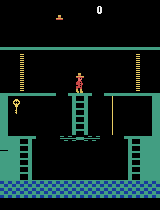
\includegraphics[width=1cm]{./imgs/mz0.png}};
		\node (frame1) [image, xshift=-0.2cm, yshift=0.2cm, opacity=0.8]
			{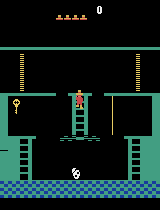
\includegraphics[width=1cm]{./imgs/mz1.png}};
		\node (frame2) [image]
			{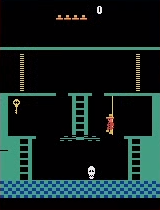
\includegraphics[width=1cm]{./imgs/mz3.png}};
		\node (frames) [fit=(frame0) (frame2), pin=above:{input sequence}] {};
		% Function
		\draw [->, thin, draw=lightgray] (frame0.east) ++(0.7,0) -- ++(2,0)
			coordinate (fn0-right);
		\draw [->, thin, draw=gray] (frame1.east) ++(0.7,0) -- ++(2,0)
			coordinate (fn1-right);
		\path (frame2.east) ++(0.7,0) edge [arrow]
			node [midway, auto=right, outer sep=0.7ex,
					pin={[pin edge=pin line]below:{unknown\\valuation function}}] {
				$f: \obsS \to \B^{\abs{\fluents}}$}
			coordinate [at end] (fn2-right) ++(2,0);
		% Output
		\begin{scope}[every matrix/.style={
			matrix of nodes, nodes in empty cells,
			row sep=-\pgflinewidth, column sep=-\pgflinewidth,
			nodes={anchor=center, draw, minimum width=1.1em, minimum height=1.1em,
				font=\footnotesize, inner sep=3pt, fill=white},
			cells={draw},
		}]
			\matrix (values0) [right=of fn0-right, nodes={draw=lightgray, thin}] {
				\\\\\\\\\\
			};
			\matrix (values1) [right=of fn1-right, nodes={draw=gray, thin}] {
				\\\\\\\\\\
			};
			\matrix (values2) [right=of fn2-right] {
				1\\1\\0\\1\\0\\
			};
		\end{scope}
		\node (values) [fit=(values0) (values2), pin={output trace}] {};
		% Constraint
		\draw (values2.east) ++(0.5,0) edge [thick, dashed]
			node [midway, auto=right, outer sep=0.7ex,
					pin=below:{temporal constraint}]
				{$\trace \models \constraintS$}
			coordinate [at end] (line-right) ++(2,0);
		\node (formula) [right=0.5cm of line-right] [pin=above:{\ldl{} formula}]
			{\constraintS};
	\end{tikzpicture}
	\caption{The trace generated by the valuation function must satisfy the
	temporal constraint.}
	\label{fig:constraints-scheme}
\end{figure}

We've just described how temporal constraints work. However, there is one
important consideration to do: these constraints are very weak. This means
that there will be lots of fluents' valuations functions that are consistent
with this specification. Consider Example~\ref{ex:door}, a feature
extractor~${f(o) \coloneqq \set{}}$ completely ignores the input and always
predicts that both fluents are false. It is wrong but it's perfectly
consistent with the specification. Similarly, many other valuation functions
that respect the DFA dynamics of Figure~\ref{fig:door-automa} will be
completely meaningless.  This may not surprise us, as most constraints can
only relate the valuation functions with each other, but they cannot force
arbitrary input--output associations. The initial and final conditions (such
as $\lnot \const{HaveKey} \land \lnot \const{DoorOpen}$ in the
Example~\ref{ex:door}) are some of the few examples that creates a strong
binding between input observations and desired fluents' output.


\section{Assumptions}

\label{sec:fluents-assumptions}

In this section, we'll list the initial choices and assumptions taken in this
work.  Of course, assumptions like these restrict the range of valuation
functions that can be learnt. However, they are essential in order to devise a
solution.  The purpose of most of them is to address the issue mentioned in
the previous section: temporal constraints are only very weak indications of
the desired meaning of the fluents. Other assumptions, instead, describe the
range of environments which the proposed model can be applied to.

First, we remember that the environments we're dealing with are video games
from the Atari collection.  So, the input space is composed of images of size
$(210, 160)$. In the following, we will always use images from this games,
because this is how environment's observations look like.

Then, we assume that each atomic proposition can be decided just from a fixed
region of the input image. In other words, to each fluent, we associate a
rectangular portion of the input and we assume that an observation of this
region is sufficient to decide the truth of the symbol. Regions can overlap
and different fluents can be defined on the same region. By restricting the
input space of the model so much, we're partially reducing the complexity of
the problem.  

\begin{example}
	In order to better understand what regions are, we anticipate one
	environment that we'll encounter in the experiments
	Section~\ref{sec:exp-breakout}: Breakout. In this famous game, the player's
	goal is to direct the ball toward the bricks. Suppose we want to learn three
	fluents~$\fluents \coloneqq \set{\const{Empty}, \const{Full},
	\const{PaddleLeft}}$, as shown in Figure~\ref{fig:assumption-ex-breakout}.
	\begin{figure}
		\centering
		\begin{tikzpicture}[
				every node/.append={font=\footnotesize},
				small arrow/.style={->, thin, >=spaced stealth'},
			]
			\node [image, outer sep=0pt] (env-br)
				{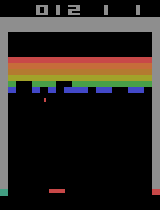
\includegraphics[height=3cm]{./imgs/br2.png}}; \&
			\begin{scope}[
					shift=(env-br.north west), x={(env-br.north east)},
					y={(env-br.south west)}]
				\draw [region box] \boxblueright node (blueright) {};
				\draw [region box] \boxpaddleleft node (paddleleft) {};
			\end{scope}
			\matrix (bluem) [matrix of math nodes, right=of blueright] {
				\const{Full} \\ \const{Empty} \\
			};
			\node (leftn) [left=of paddleleft] {$\const{PaddleLeft}$};
			\draw [small arrow] (bluem-1-1) -- (blueright-|env-br.east);
			\draw [small arrow] (bluem-2-1) -- (blueright-|env-br.east);
			\draw [small arrow] (leftn) -- (paddleleft-|env-br.west);
		\end{tikzpicture}
		\caption{Fluents and regions for the environment Breakout in
		Example~\ref{ex:assumption-ex-breakout}.}
		\label{fig:assumption-ex-breakout}
	\end{figure}
	The region associated to each of these symbols is indicated with an orange
	box. $\const{PaddleLeft}$ should be true when the paddle is inside the
	area on the left; $\const{Empty}$ and $\const{Full}$ should be true
	respectively when all the bricks, or no bricks, inside the region have been
	shot down.
	\label{ex:assumption-ex-breakout}
\end{example}

As it may be clear from this example, the regions also help to do something
that would be impossible in logic: indicate to which portion of the input the
fluents refer. Also, we should choose each region as a small selection of
the image in which the condition we'd like to extract is \emph{visually
evident}: to different valuations should correspond noticeable differences
in the region. In the following sections, we'll refine what we mean by
``noticeable''. Essentially, we mean that the model must be able to learn an
encoding that captures the properties we're interested in. Unfortunately,
this is not something that can be described with extreme precision, in machine
learning. We'll discuss this issue in Section~\ref{sec:encoding-what-learns}.

Due to these fixed regions, this method is only applicable to games with a
fixed view of the scene. If every object in the image were moving, we
couldn't apply the simplification of static regions. Few examples of games
that respect this constraint are: Breakout, Mr.~Pac-Man, Video Pinball, Pong.
We'll also experiment with Montezuma's Revenge, but we'll limit to the first
room.

In Section~\ref{sec:fluents-limitations},
``\nameref{sec:fluents-limitations}'', we'll suggest few ideas about how many
of these limitations might be relaxed.


\section{General structure of the model}

\label{sec:model-structure}

In this section, we introduce the general structure of the model that we
propose in this thesis. The remaining parts of the chapter will cover all the
details and definitions.

As we already know, temporal constraints can exclude many inconsistent
assignments but they are only weak indications about the desired valuation
functions. By assuming regions, we've strongly reduced the size of the input
space, hence of the possible functions. Still, the problem is only mitigated.
To address this issue, we propose to learn each valuation function from an
encoding vector that represents the region of interest, rather than from the
pixel values directly. An encoding is a low-dimensional vector that represents
a more complex input. So, we might use this vector in place of the original
input in order to simplify the learning process of the valuation function.

An encoding can be viewed as a lossy compression of the input. The meaning of
the encoding vector depends on the specific model, which will be presented in
Section~\ref{sec:encoding}. Here, we only want to highlight that all input
images that are considered similar according to the model will correspond to
the same encoding vector. Hence, these images will produce the same
interpretation for the fluents. However, this is certainly a desirable effect:
the encoder can extract few relevant indicators from which we can compute the
fluents' values, while noises and tiny variations of the input will be
ignored.

So, the model that we propose is a function composed of two consecutive parts:
an array of \emph{encoders} and an array of \emph{Boolean functions}.  This
scheme is illustrated in Figure~\ref{fig:model-scheme}.
\begin{figure}
	\centering
	\begin{tikzpicture}[
			node distance=0.7cm,
			every label/.style={font=\scriptsize},
		]

		% Input
		\node [image] (frame)
			{
\includegraphics[height=2cm]{./imgs/br0.png}};
		\node [dot, right=0.7cm of frame] (input) {};

		% Encoders
		\matrix [
			right=of input, nodes={anchor=center},
			row sep=0.5cm, column sep=0.5cm,
		] (encoders) {
			\node [block] (encoder1) {Encoder\\(region 1)}; \&
			\node [dot] (encoded1) {}; \\
			\node [block] (encoder2) {Encoder\\(region 2)}; \&
			\node [dot] (encoded2) {}; \\
		};

		% Boolean functions & output
		\matrix [
			right=of encoders, nodes={anchor=center},
			row sep=0.3cm, column sep=1cm, label distance=0.4cm,
		] (boolfns) {
			\node [block] (boolfn1) {Boolean fn 1}; \&
			\node [label=right:Fluent 1] (output1) {0}; \\
			\node [block] (boolfn2) {Boolean fn 2}; \&
			\node [label=right:Fluent 2] (output2) {1}; \\
			\node [block] (boolfn3) {Boolean fn 3}; \&
			\node [label=right:Fluent 3] (output3) {0}; \\
		};

		% Output
		\node [draw, rectangle, gray, inner sep=0pt, fit=(output1) (output3)
			] (outputs) {};

		% Flow
		\draw (frame) to (input);
		\draw [->] (input) edge (encoder1) edge (encoder2);
		\draw (encoder1) to (encoded1);
		\draw (encoder2) to (encoded2);
		\draw [->] (encoded1) edge (boolfn1.west) edge (boolfn2.west);
		\draw [->] (encoded2) edge (boolfn3.west);
		\draw [->] (boolfn1) to (output1);
		\draw [->] (boolfn2) to (output2);
		\draw [->] (boolfn3) to (output3);

		% Models
		\begin{pgfonlayer}{below}
			\node (model) [
				fit=(input) (encoders) (boolfn1) (boolfn3),
				draw=blue!30!gray, fill=blue!40!gray!20!white,
				inner sep=0.2cm, label=above:{\normalsize Model},
			] {};
		\end{pgfonlayer}

		% Annotations
		\coordinate (annotations y) at ($(model.south)+(0,-0.8)$);
		\begin{pgfonlayer}{below}
			\node (input-annotation) at (input|-annotations y) {Input};
			\node (encoding-annotation) at (encoded1|-annotations y) {Encodings};
			\node (outputs-annotation) at (outputs|-annotations y) {Predictions};
			\draw [pin line] (input) -- (input-annotation);
			\draw [pin line] (encoded1) -- (encoding-annotation);
			\draw [pin line] (outputs) -- (outputs-annotation);
		\end{pgfonlayer}
	\end{tikzpicture}
	\caption{The model is composed by a sequence of encoders and a set of
	Boolean functions.}
	\label{fig:model-scheme}
\end{figure}
Let's assume that the set~$\fluents$ of fluents to learn is given, along with
their associated regions. We create an encoder for each region and a Boolean
function for each symbol in~$\fluents$. There might be less encoders than
Boolean functions, because multiple fluents can share the same region.
This scheme has two encoders and three Boolean functions (just like the model
associated to the example in Figure~\ref{fig:assumption-ex-breakout}). Of
course, that is just a specific instance. There will be as many parts as are
needed.

To summarize:
\begin{enumerate}
	\item The input frame is cropped around each region;
	\item Each small image is transformed with its own encoder;
	\item Each Boolean function computes the value for one fluent from the
		corresponding encoding vector.
\end{enumerate}


\section{Encoding}

\label{sec:encoding}

The encoder is a Machine Learning model that is trained in an unsupervised
way, whose purpose is to convert the input of one region to the associated
low-dimensional representation. The model we've selected for this role is the
Deep Belief Network. As we will see, this choice is mainly motivated by the
output produced by this model, which is a vector of binary features. In the
following, we'll thoroughly describe this model, and discuss why a binary
output is so important.

Since the layers of a Deep Belief Network are a specific type of Markov Random
Field, it is better to quickly review these first. This will allow us to
better understand the goal and properties of the final encoder.


\subsection{Markov Random Fields}
% TODO: ref

In the previous chapters, we have sometimes used Directed Graphical Models
(for example in Figure~\vref{fig:mdp}). These are probabilistic models in
which directed arcs represent known conditional probabilities between two
variables. Here, instead, we'll adopt a different kind of formalism:
\emph{Undirected Graphical Models} (UGMs)\nomenclature{UGM}{Undirected
Graphical Models}, which are also called \emph{Markov Random Fields}
(MRFs)\nomenclature{MRF}{Markov Random Fields}.

A UGM is an undirected graph, where variables are represented by nodes, as
usual, and undirected arcs connect variables which are directly dependent.
A missing edge means that two variables are conditionally independent given
the others. For example, in Figure~\ref{fig:mrf}, $x_1$ and $x_4$ are
dependent variables, but they become conditionally independent if $x_2$ is
observed.
\begin{figure}
	\centering
	\begin{tikzpicture}[semithick]
		\graph [
			spring layout,
			empty nodes, nodes=node,
			horizontal=x2 to x4,
		] {
			x1 [label=left:$x_1$] -- x2 [label=above:$x_2$] -- 
				x3 [label=left:$x_3$] -- x1,
			x2 -- x4 [label=right:$x_4$]
		};
	\end{tikzpicture}
	\caption{A small MRF where: $x_1 \not\perp x_4$, but $x_1 \perp x_4 \given
	x_2$.}
	\label{fig:mrf}
\end{figure}
In this and the following graphs, we assume that each node represents a scalar
quantity. Vectorial quantities will be indicated in bold fonts.

MRFs are very convenient when we what to express that two variables are
related, but we can't establish any causal relation between them. Consider,
for example, the noisy pixels of an image. The values of neighbouring pixels
are clearly dependent, as they are related by the subject of the image, but we
can't establish any useful conditional probability between the two.

In every MRF, the joint probability of all the variables can be expressed as:
\begin{equation}
	p(\x \given \params) \propto
		\prod_{c \in \setSym{C}} \psi_c(\x_c; \params_c)
\end{equation}
where each $c \in \setSym{C}$ is a maximal clique of the graph, and each
function $\psi_c$ computes how likely is the observation of variables~$\x_c$,
according to the parameters~$\params_c$. The joint probability is only
proportional to that quantity, because one normalizer has been omitted. As an
example, the joint probability for Figure~\ref{fig:mrf} can be written:
\[
	p(x_1, x_2, x_3, x_4 \given \params) \propto
	\psi_1(x_1, x_2, x_3; \params_1) \, \psi_2(x_2, x_4; \params_2)
\]

Therefore, a model for a MRF is fully defined by two factors: the structure of
the graph, and the functions~$\psi_c$. While the former strongly depends on
the process to be modelled, we can present the most common choice for the
latter. First, let's rewrite each term as:
\begin{equation}
	\psi_c(\x_c; \params_c) \coloneqq \exp(-E(\x_c; \params_c))
	\label{eq:ugm-energy-based}
\end{equation}
for some function~$E$. $E$ is called the \emph{energy function}. Since it is
inversely correlated to the probability, it is high for unlikely
configurations of variables and low for very probable configurations
(according to the model parameters, of course). Due to this property, it is
sometimes a very useful indication of the final probability\footnote{Computing
the exact probability $p(\x \given \params)$, as many other quantities, is
intractable for generic UGMs, because often we won't be able to compute the
normalizer}.  Usually, the energy function is of the simplest kind, a linear
combination: $E(\x_c; \params_c) \coloneqq -\params_c^T \basisfun_c(\x_c)$,
for some basis function~$\basisfun_c$. In the following, we'll assume this
form.

As we may recognize, in a MRF there is no output. We're not trying to learn an
input--output function. Training a model means to find the optimal parameters
$\optimal\params$ that maximize the probability of the input samples. The
trained model should represent the probability distribution of the input data,
as closely as possible. This is clearly different from supervised learning.

Let's denote with $\dataset$ a dataset of training samples, $\dataset
\coloneqq \set{\x\group{i}}$, and with $l(\params)$ the log-probability of the
dataset according to the model, $l(\params) \coloneqq \log p(\dataset \given
\params)$. The optimal parameters are those maximizing the likelihood
$l(\params)$. So, we may approach this solution by following the positive
gradient of the likelihood. The gradient of the likelihood, with respect to
each group $c$ of parameters, is~\footnote{ The function $\basisfun_c$ only
receives the values of the clique $c$.  In the following equation, we write
$\x$ instead of $\x_c$, to ease the notation.}:
\begin{equation}
	\frac{\partial l}{\partial \params_c} = \E_{\x' \sim \dataset}
	\bigl[\basisfun_c(\x') \bigr] - \E_{\x} \bigl[\basisfun_c(\x) \bigr]
	\label{eq:ugm-gradient}
\end{equation}
The two parts compute the expected value of same quantity according to a
different distribution of~$\x$. The positive term simply stands for the
average value of that quantity, computed from the samples in the training
dataset; while in the right-most term, we take an expectation on $\x$
according to the distribution induced by the model.

We'll end this quick review of MRFs, by discussing the role of latent
variables. As we already know from the comparison between MDPs and POMDPs,
probabilistic models that include some unobservable variables can be much more
expressive than the others. Such variables are referred to as \emph{latent}
variables, or simply \emph{hidden} variables. The latent variables of a model
can be a very effective explanation of the visible quantities. For example,
the states of a POMDPs can explain even very complex observations. Similarly,
some latent variables that represent the subject of an image are a clear cause
for the observed pixel values. Connecting the visible units directly would
require a much more complex model. Latent units in a MRF do not define such
causal relation, but they allow a very similar expressiveness.

We partition the variables as $\x = (\bv, \bh)$, where $\bv$ and $\bh$ denote
the visible and hidden variables, respectively.  A model with latent variables
can be trained very similarly to what we've seen above. The only difference is
that we need to always take the expectation on $\bh$ according to the model,
because they will never be observed in the dataset:
\begin{equation}
	\frac{\partial l}{\partial \params_c} = \E_{\bv \sim \dataset,\bh}
	\bigl[\basisfun_c(\bv, \bh)\bigr] - \E_{\bv,\bh} \bigl[\basisfun_c(\bv,
	\bh)\bigr]
	\label{eq:ugm-po-gradient}
\end{equation}


\subsubsection*{Restricted Boltzmann Machine}

The specific model that we'll use is the \emph{Restricted Boltzmann Machine}
(RBM)\nomenclature{RBM}{Restricted Boltzmann Machine}. An RBM is a MRF
composed of a visible and a hidden layer. Its graph is shown in
Figure~\ref{fig:rbm}.
\begin{figure}
	\centering
	\begin{tikzpicture}[
		semithick, node distance=1.2cm and 1.2cm, anchor=center
	]

	\node [hidden node, label=above:$h_1$] (h1) {};
	\node [hidden node, label=above:$h_2$, right=of h1] (h2) {};
	\node [right=of h2] (dots1) {\dots};
	\node [hidden node, label=above:$h_H$, right=of dots1] (hK) {};

	\node [node, label=below:$v_1$, below=of h1, xshift=-0.7cm] (v1) {};
	\node [node, label=below:$v_2$, right=of v1] (v2) {};
	\node [node, label=below:$v_3$, right=of v2] (v3) {};
	\node [right=of v3] (dots2) {\dots};
	\node [node, label=below:$v_V$, right=of dots2] (vR) {};

	\graph {{(h1), (h2), (hK)} --[complete bipartite] {(v1), (v2), (v3), (vR)}};
	\end{tikzpicture}
	\caption{The UGM of a Restricted Boltzmann Machine. Gray nodes are latent
	variables.}
	\label{fig:rbm}
\end{figure}
As we can see, there are no connections between variables of the same layer,
and every clique has two nodes. So, the joint probability is simply:
\begin{equation}
	p(\bv, \bh) \propto \prod_{i=1}^{V} \prod_{j=1}^{H} \psi_{ij}(v_i, h_j)
\end{equation}
with one function $\psi_{ij}$ for each arc $(v_i, h_j)$. This simplification,
along with other nice properties, are possible because there is just one
hidden layer. This is why it is said ``restricted''.

The classic RBM, which is the one we'll use here, assumes that all variables
are binary: $v_i, h_j \in \set{0,1}$. It defines the following energy
function:
\begin{equation}
	E(\bv,\bh; \params) \coloneqq -( \bv^T \linparmat \bh + \bv^T \bvec{b} +
	\bh^T \bvec{c})
\end{equation}
where the weights $\linparmat$ and biases $\bvec{b}$, $\bvec{c}$ are all the
model's parameters~$\params$.

% TODO: extend with 1 or maybe leave biases?
% TODO: conditional probabilities
% TODO: gradient of the log



% TODO: training algorithm.


\subsection{Deep Belief Networks}

% TODO: nomenclature

\label{sec:dbn}

% TODO
%Encoder: the model, how it works, what does it learn, size of the encoding.
%
%References:
%Training Restricted Boltzmann Machines and Deep Belief Neworks
%\cite{bib:rbm-training}\cite{bib:ml-book-murphy}.

\subsection{What does it learn}

\label{sec:encoding-what-learns}

% TODO: large region for room
% Consider, for example, the region of the fluents $\const{Full}$ and
% $\const{Empty}$ of Figure~\ref{fig:assumption-ex-breakout}. The most evident
% change in that area are the disappearing bricks; we won't be able to learn a
% fluent $\const{BallInside}$ that becomes true when the ball is inside the
% region.

\section{Boolean functions}

The fluents are true in a set of those configurations.

\subsection{Learning with genetic algorithms}

Ideas from concept learning; genetic algorithm.

References:
Genetic Algorithms for Concept learning\cite{bib:ga-for-concepts},
Genetic Algorithms review\cite{bib:ga-mutations-review}.

\subsection{Boolean rules}

Representation of boolean functions and training details.

\section{Limitations and improvements}

\label{sec:fluents-limitations}

% TODO: strong grounding of few symbols? Supervised?
% TODO: different rooms?
% TODO: unsure about representable with conjunction, because DBN is
%		unsupervised
% TODO: no guarantees but easy to check
